\chapter{Research Methods}
\lhead{\emph{Research Methods}}

This chapter provides information about the research methods used in the project. Before conducting a series of experiments to explore and evaluate machine learning methods, it was needed to decide on how are these algorithms are going to be implemented and evaluated. The list of following things had to be decided first: \begin{enumerate}
  \item Choose a programming language.
  \item Choose machine learning libraries.
  \item Choose the evaluation method for evaluating the performance of machine learning algorithms
\end{enumerate}The choices made and the reasoning behind them are going to be explained next.

\section{Choice of a Programming Language}

 It was chosen to use Python programming language for implementing this project. The language was chosen because it is one of the most popular languages used by machine learning researchers and developers. It is also free and open sourced. Since Python is an interpreted language, code written in Python can be executed on multiple different platforms without having a need to change anything in the code. Thanks to Python's popularity, there are many publicly available and open sourced packages with efficient implementation of machine learning algorithms, that can be downloaded.

Availability of scientific computing tools for Python was also one of the main reasons why this language was chosen. Scientific Python libraries used in this project were Matplotlib, NumPy, IPython and Jupyter Notebook \citep{scipy}. Matplotlib provided an ability to plot graphs, images, and tables. NumPy was used for efficient arithmetical operations with matrices. IPython is a System for an interactive scientific computing \citep{ipython}. It allowed working with code interactively. IPython allows executing only the parts of a program without having a need to re-execute the full code of the program. This function was very beneficial. Some of the operations like loading the dataset, resizing the images in the dataset can take a long time to run, but in Ipython dataset is only needed to load once. Then, it is saved to the memory and can be reused in other blocks of code. Jupyter Notebook is an Ipython wrapper that launches a HTTP server. It allowed to execute Python code in a web browser and to save the results as HTML pages \autoref{fig:jupyter}. Combined, these libraries allowed to interactively explore the data with the ability to plot graphs, tables and to visualize the results.

The alternative language that was also considered was Matlab. Matlab is a domain specific programming language that was designed specifically for matrix programming. It also includes image processing and machine learning toolboxes. Because this language was developed for the particular purpose, machine learning and image processing functions are easier to use in Matlab than in Python. However, Matlab is a closed source language. It also only supports some platforms, where Python code can be run in almost any computing environment. Because of these disadvantages, it was decided to use Python.

\begin{figure}[ht]
\centering
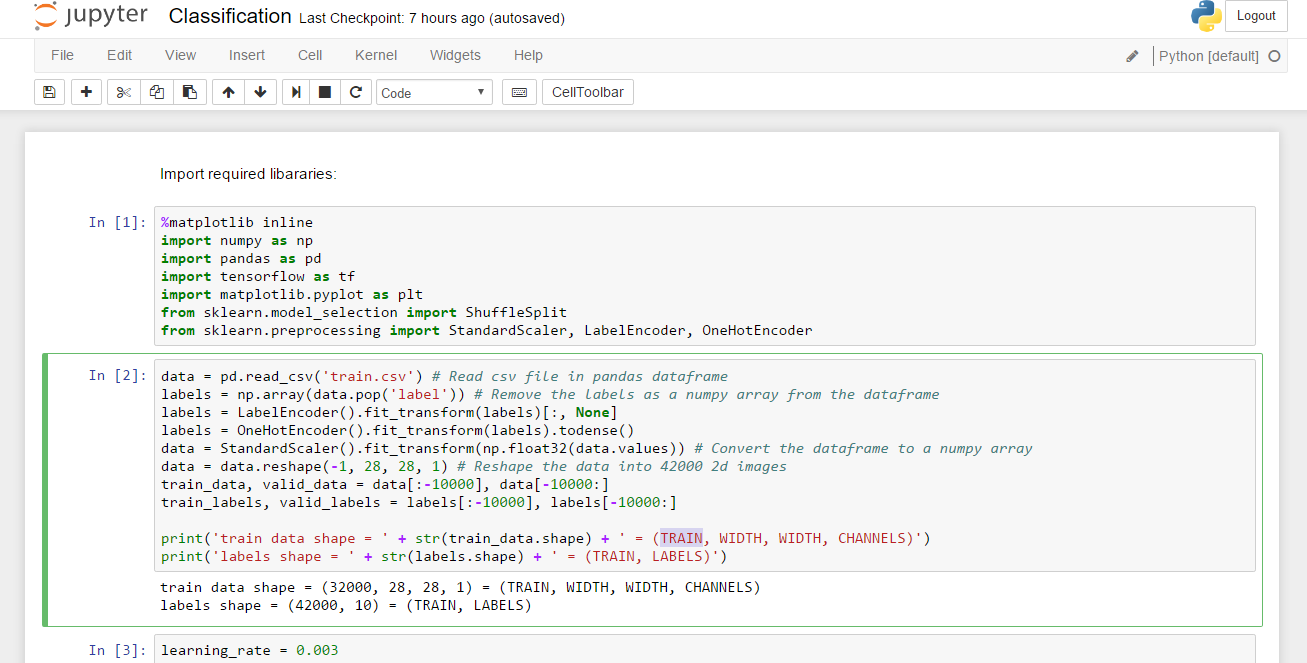
\includegraphics[width=14cm]{Figures/c3/c3jupyter.PNG}
\caption{Example of a Jupyter Notebook}
\label{fig:jupyter}
\end{figure}


\section{Choice of Machine learning libraries}

\subsection{Why was a Machine Learning Library Needed}

It is possible to implement machine learning algorithms without using any additional libraries. However, there are many benefits provided by using a  machine learning library. Algorithms provided in machine learning libraries often can be more efficient. It also takes a less time to adapt a provided algorithm for a task than to write a particular algorithm for it. Because of that, it was decided to research what machine learning libraries exist for Python.

\subsection{Library Used for Machine Learning }

Sckit-learn python package was chosen as a library for working with machine learning models. This package provides state-of-the-art implementations of many well-known machine learning algorithms. It also has an easy-to-use interface tightly integrated with the Python language \citep{pedregosa2011scikit}. Large parts of this module are written in c or C++. Because C and C++ are much faster than Python, it makes algorithms run faster compared to a standard Python implementation. Sckit\-learn machine learning algorithms are high-level API's.  A programmer does not need about how these algorithms are implemented. Nevertheless, algorithms provided in this package are very flexible and can be configured to programmer's needs \citep{buitinck2013api}.

In the case of food image classification, the main advantages that Sckit-learn provided were the fact that it used same data input format for every machine learning algorithm and that parameters of algorithms could be easily configured to make classifiers work on image classification problem.


\section{The Evaluation Method for the Classification Algorithms}

The key indicator of performance in the classification task is a classification accuracy. Accuracy is calculated by dividing the number of correct predictions by the total number of predictions. By calculating and comparing accuracy scores for every machine learning algorithm tried, the best food image classification technique was found.

Other helpful performance indicators used to evaluate a classification performance when parameters of classification algorithms were tuned confusion matrix, precision, recall and f measure. Confusion matrix shows how often and what classes are misclassified as other classes. Precision it the total number of elements classified correctly divided by a total number of elements that were classified as that class. A recall is the total number of items classified correctly divided by a total number of items of that type in the database. A graphical ilustration of presicion and recall mesures is shown in \autoref{fig:p}.  F-measure is a measure combined from precision and recall according to a formula \( F = 2 \frac{Recall \times Precision }{Recall  +  Precision} \)   \citep{ting2011}. 


\begin{figure}[ht]
\centering
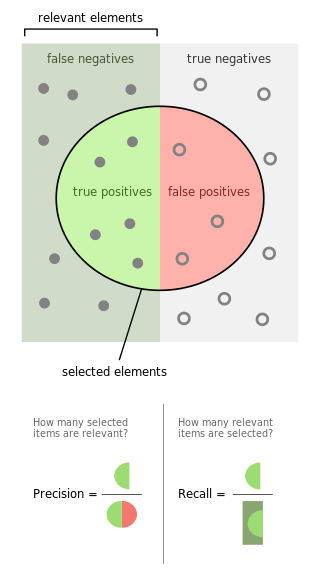
\includegraphics[width=5cm]{Figures/c3/p.png}
\caption{Graphical illustration of the precision and recall \cite{wiki:p}}
\label{fig:p}
\end{figure}


\section{Summary}
In this chapter reasoning behind a chosen programming language and machine learning library used was provided. It was also described how image classifiers that use machine learning algorithms are going to be built. Finally, methods for evaluating the performance of classification algorithms were discussed, and accuracy score was picked as the primary method for performance evaluation. In the following chapter, accumulation of a food image dataset is going to be discussed.